

\tikzset{every picture/.style={line width=0.75pt}} %set default line width to 0.75pt        

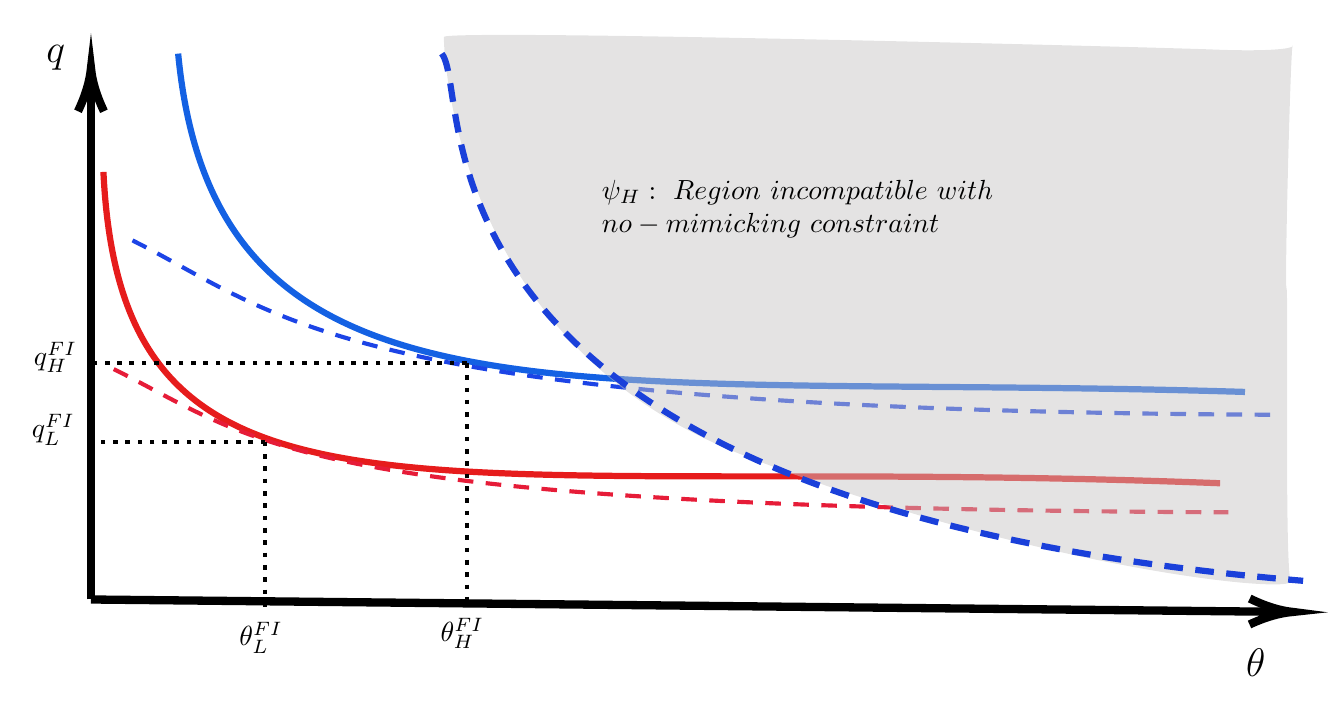
\begin{tikzpicture}[x=0.75pt,y=0.75pt,yscale=-1,xscale=1]
%uncomment if require: \path (0,326); %set diagram left start at 0, and has height of 326

%Straight Lines [id:da40072496639048816] 
\draw [line width=3]    (36,273) -- (610,278.95) ;
\draw [shift={(615,279)}, rotate = 180.59] [color={rgb, 255:red, 0; green, 0; blue, 0 }  ][line width=3]    (20.77,-6.25) .. controls (13.2,-2.65) and (6.28,-0.57) .. (0,0) .. controls (6.28,0.57) and (13.2,2.66) .. (20.77,6.25)   ;
%Straight Lines [id:da592043984950475] 
\draw [line width=3]    (36,273) -- (36,22) ;
\draw [shift={(36,17)}, rotate = 90] [color={rgb, 255:red, 0; green, 0; blue, 0 }  ][line width=3]    (20.77,-6.25) .. controls (13.2,-2.65) and (6.28,-0.57) .. (0,0) .. controls (6.28,0.57) and (13.2,2.66) .. (20.77,6.25)   ;
%Curve Lines [id:da9360675954512778] 
\draw [color={rgb, 255:red, 20; green, 97; blue, 227 }  ,draw opacity=1 ][line width=2.25]    (78,10) .. controls (96,199) and (268,163) .. (592,173) ;
%Curve Lines [id:da9943224819031027] 
\draw [color={rgb, 255:red, 230; green, 28; blue, 28 }  ,draw opacity=1 ][line width=2.25]    (42,67) .. controls (51,255) and (195,202) .. (580,217) ;
%Curve Lines [id:da6762600522165454] 
\draw [color={rgb, 255:red, 28; green, 68; blue, 230 }  ,draw opacity=1 ][line width=1.5]  [dash pattern={on 5.63pt off 4.5pt}]  (56,100) .. controls (129,136.5) and (156,182) .. (607,184) ;
%Curve Lines [id:da032357010381118156] 
\draw [color={rgb, 255:red, 230; green, 28; blue, 56 }  ,draw opacity=1 ][line width=1.5]  [dash pattern={on 5.63pt off 4.5pt}]  (47,162) .. controls (120,198.5) and (133,229) .. (584,231) ;
%Straight Lines [id:da30034505282826984] 
\draw [line width=1.5]  [dash pattern={on 1.69pt off 2.76pt}]  (217,159) -- (217,275) ;
%Straight Lines [id:da399603317665826] 
\draw [line width=1.5]  [dash pattern={on 1.69pt off 2.76pt}]  (217,159) -- (35,159) ;
%Shape: Polygon Curved [id:ds04927104483806066] 
\draw  [draw opacity=0][fill={rgb, 255:red, 198; green, 196; blue, 196 }  ,fill opacity=0.48 ] (206,2) .. controls (206,-2) and (552,7) .. (576,8) .. controls (600,9) and (616,8) .. (615,6) .. controls (614,4) and (611,123) .. (612,123) .. controls (613,123) and (611,257) .. (614,264) .. controls (617,271) and (489,258) .. (349,203) .. controls (209,148) and (206,6) .. (206,2) -- cycle ;
%Straight Lines [id:da1316418064859366] 
\draw [line width=1.5]  [dash pattern={on 1.69pt off 2.76pt}]  (120,197) -- (120,277) ;
%Straight Lines [id:da26757400472013826] 
\draw [line width=1.5]  [dash pattern={on 1.69pt off 2.76pt}]  (120,197) -- (40,197) ;
%Curve Lines [id:da7998201330100672] 
\draw [color={rgb, 255:red, 26; green, 64; blue, 218 }  ,draw opacity=1 ][line width=2.25]  [dash pattern={on 6.75pt off 4.5pt}]  (205,10) .. controls (221,30) and (176,227) .. (620,264) ;

% Text Node
\draw (591,295.4) node [anchor=north west][inner sep=0.75pt]  [font=\Large]  {$\theta $};
% Text Node
\draw (13,4.4) node [anchor=north west][inner sep=0.75pt]  [font=\Large]  {$q$};
% Text Node
\draw (203,280.4) node [anchor=north west][inner sep=0.75pt]    {$\theta _{H}^{FI}$};
% Text Node
\draw (7,147.4) node [anchor=north west][inner sep=0.75pt]    {$q_{H}^{FI}$};
% Text Node
\draw (274,67.4) node [anchor=north west][inner sep=0.75pt]    {$ \begin{array}{l}
\psi _{H} :\ Region\ incompatible\ with\\
no-mimicking\ constraint
\end{array}$};
% Text Node
\draw (106,282.4) node [anchor=north west][inner sep=0.75pt]    {$\theta _{L}^{FI}$};
% Text Node
\draw (6,182.4) node [anchor=north west][inner sep=0.75pt]    {$q_{L}^{FI}$};


\end{tikzpicture}